\documentclass[serif,9pt]{beamer}
\setbeamertemplate{navigation symbols}{}

\usepackage[utf8]{inputenc}
\usepackage[T1]{fontenc}
\usepackage[catalan]{babel}

\usetheme{Warsaw}
\usecolortheme{seahorse}

\beamersetuncovermixins{\opaqueness<1>{25}}{\opaqueness<2->{15}}

%\AtBeginSection[]
%{
%  \begin{frame}<beamer>
%    \frametitle{Continguts}
%    \tableofcontents[currentsection]
%  \end{frame}
%}

\setcounter{tocdepth}{1}

\begin{document}

\title[Quadriga]{Quadriga: Plataforma de Programació en Sistemes d'Entitats, per al desenvolupament de Videojocs}  
\author{Isaac Serrano}
\institute{Universitat Autònoma de Barcelona}
\date{7 de Juliol del 2011}

\begin{frame}
\titlepage
\end{frame}

\begin{frame}
\frametitle{Continguts}
\tableofcontents
\end{frame}

\section{Introducció}

  \subsection{Motivació}

    \begin{frame}\frametitle{Motivació}
     \begin{itemize}
      \item Augment de la complexitat en la creació de videojocs.\bigskip
      \item Surt més a compte comprar un motor que crear-lo. \bigskip
      \item Molts motors disponibles, fins i tot lliures (Ogre, jMonkeyEngine, etc.).\bigskip
      \item Com crear un joc sobre aquests motors? Mòdul de Lògica.
     \end{itemize}
    \end{frame}
    
    % 

    \begin{frame}\frametitle{Esquema Motor de Videojoc}
      \begin{center}
        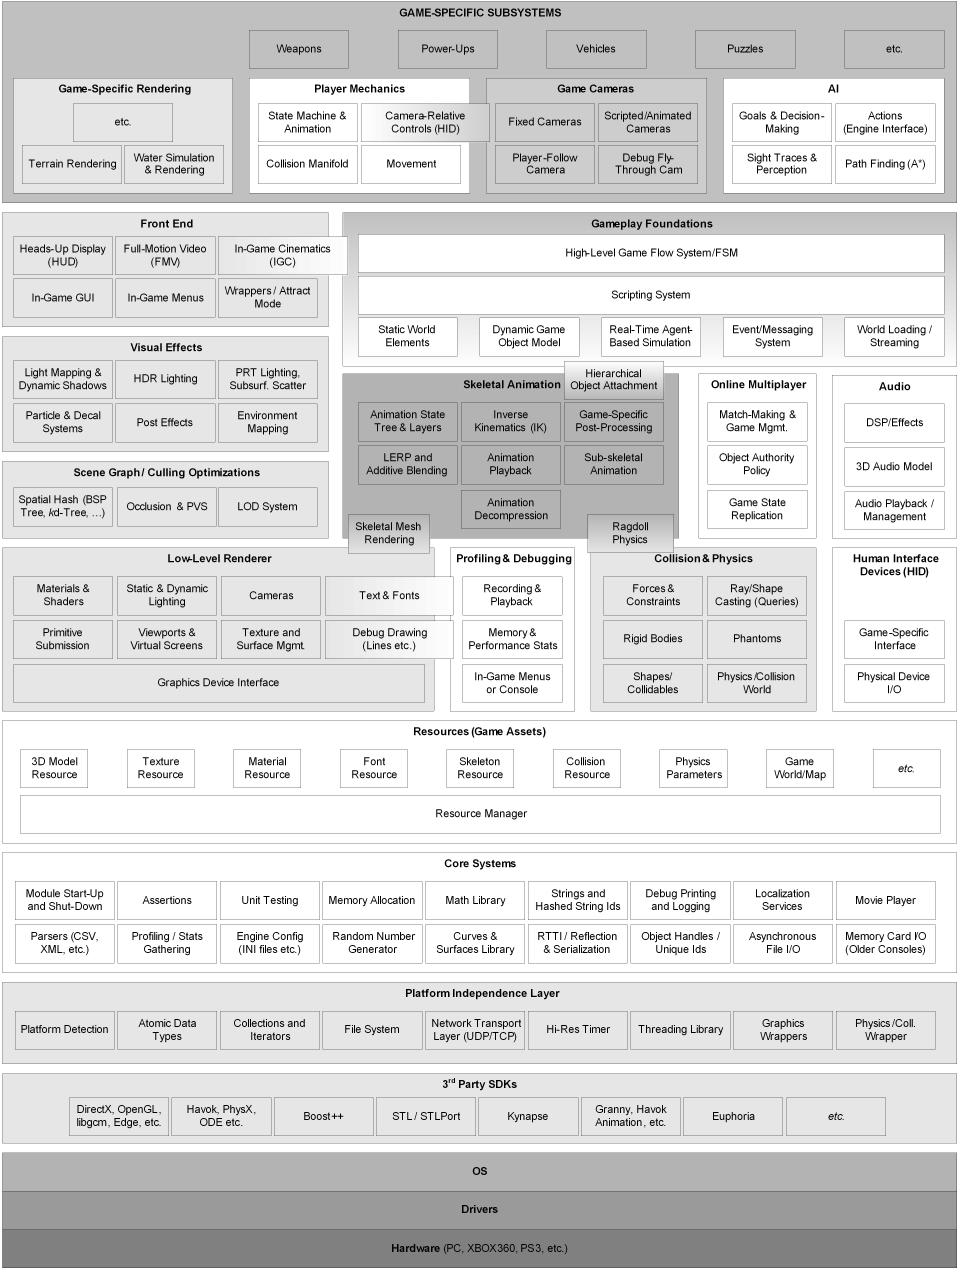
\includegraphics[width=0.50\textwidth]{./img/Fig-RuntimeArch.jpg}
      \end{center}
    \end{frame}

    \begin{frame}\frametitle{Mòdul de Lògica}
      \begin{itemize}
        \item Ha de permetre crear els objectes del joc (arbres, vegetació, monstres, nivells, portes, herois, objectes d'inventari, triggers, seqüències de càmera...) i el seu comportament (renderitzar, cerca de camins, animar, fer decisions d'IA...).\bigskip
        \item Ha de crear/destruir els objectes en el joc i coordinar els missatges entre ells.\bigskip
        \item Ha de mantenir una BBDD dels objectes actius, i crear-se a partir d'una altra BBDD estàtica (que defineix el joc).\bigskip
        \item Esquemàticament, {\bf tots} els jocs tenen això d'una manera o altra.
      \end{itemize}
    \end{frame}

    \begin{frame}\frametitle{Esquema original}
      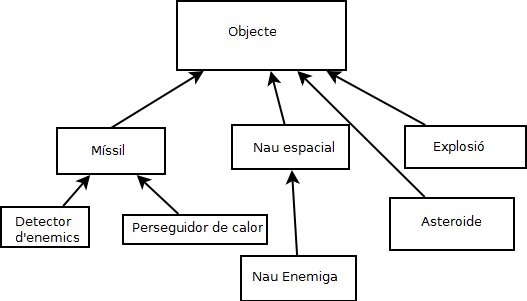
\includegraphics[width=1.00\textwidth]{./img/DiagramaObjectes1.png}
    \end{frame}

    \begin{frame}\frametitle{Refacció}
      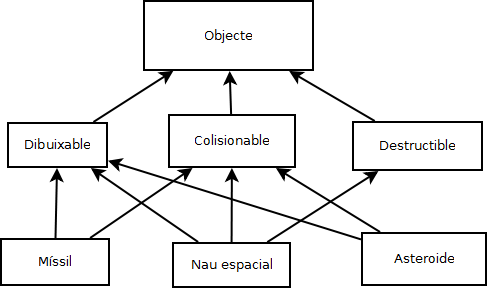
\includegraphics[width=1.00\textwidth]{./img/DiagramaObjectes2.png}
    \end{frame}

    \begin{frame}\frametitle{Refacció en Components}
      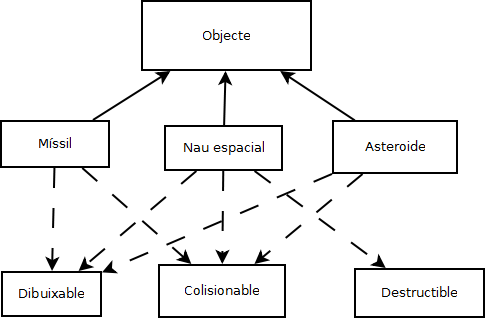
\includegraphics[width=1.00\textwidth]{./img/DiagramaObjectes3.png}
    \end{frame}
    
  \subsection{Objectius}

    \begin{frame}\frametitle{Objectius}
      Crear un mòdul de Lògica.
      \begin{itemize}
        \item Dirigit per dades, poder prescindir dels enginyers.
        \item Open Source.
        \item Multi-plataforma.
        \item Paral·lelitzable.
      \end{itemize}
    \end{frame}

\section{Desenvolupament}

  \subsection{Disseny}
  
    \begin{frame}\frametitle{Desenvolupament}
      \includegraphics[width=1.00\textwidth]{./img/EsquemaExecució.png}
    \end{frame}

  \subsection{Llenguatge}

    \begin{frame}\frametitle{Disseny}
      \begin{itemize}
        \item Crear un llenguatge de programació, Quadriga. 
        \begin{itemize}
          \item Components.
          \item Sistemes.
          \item Events.
          \item Prototips.
          \item Thread, Main.
        \end{itemize}
        \item Crear un entorn d'execució: dirigir events, mantenir la BBDD.
      \end{itemize}
    \end{frame}
  
  \subsection{Compilador}
  
    \begin{frame}\frametitle{Compilador}
      \begin{itemize}
        \item Desenvolupat amb JavaCC a partir de la gramàtica de Java 1.5. \bigskip
        \item El compilador crea un arbre sintàctic i aquest s'executa. \bigskip
        \item El compilador també crea la base de dades, específica per al joc.
      \end{itemize}
    \end{frame}
  
  \subsection{Model de dades}
    
    \begin{frame}\frametitle{Model de dades}
      \begin{itemize}
        \item Relacionar cada entitat (objecte del joc) amb els seus component i les dades corresponents. \bigskip
        \item Informar a cada sistema de quines entitats ha de modificar. \bigskip
        \item Trobar les entitats/sistemes afectats a l'hora de llençar un event i facilitar la seva recepció. \bigskip
        \item Mantenir dades d'iteracions anteriors per poder detectar noves incorporacions i baixes de sistemes.
      \end{itemize}
    \end{frame}
    
  \subsection{Entorn d'execució}
    
    \begin{frame}\frametitle{Entorn d'execució}
      \begin{itemize}
        \item Treballa directament a la JVM. Permet usar classes escrites Java sense dificultats.\bigskip
        \item Conté una base de dades. Usa HSQLDB i permet guardar tipus primitius i classes {\em Seriallizable}.\bigskip
        \item S'encarrega de la creació i destrucció d'elements, de la modificació de dades i de la comunicació amb events.
      \end{itemize}
    \end{frame}

\section{Resultats}

  %Tetris
  \begin{frame}\frametitle{Resultats}
    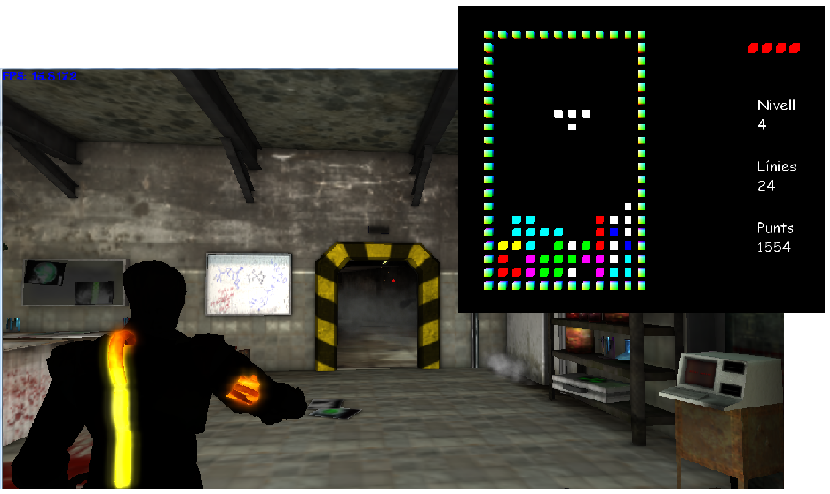
\includegraphics[width=1.00\textwidth]{./img/Screens.png}
  \end{frame}

\section{Conclusions i Millores}

  \begin{frame}\frametitle{Conclusions}
    \begin{itemize}
      \item S'ha dissenyat un llenguatge de programació anomenat Quadriga. Se n'ha programat un compilador, un intèrpret i entorn d'execució. \bigskip
      \item S'ha creat una base de dades especificada dinàmicament (resultat de la compilació). \bigskip
      \item S'ha implementat un joc d'exemple basat en el clàssic {\bf Tetris}. \bigskip
      \item S'ha dissenyat un model de llibreria tal que sigui fàcil de transportar a altres plataformes (fins i tot plataformes mòbils) emprant les últimes tècniques de renderitzat (mitjançant els {\em Shaders} d'OpenGL 2.0).
    \end{itemize}
  \end{frame}
  
  \begin{frame}\frametitle{Millores}
    \begin{itemize}
      \item Fer millores de rendiments tals com la compilació del llenguatge a bytecode. \bigskip
      \item Ampliar la llibreria estàndard per incloure la funcionalitat de so i joc en xarxa. \bigskip
      \item Crear un plug-in de la {\bf IDE} {\em Eclipse} per a desenvolupar i debugar més fàcilment.
    \end{itemize}
  \end{frame}

\begin{frame}
\frametitle{}
\titlepage
\end{frame}

\end{document}